% --------------------------------------------------------------------------- %
% Poster for the ECCS 2011 Conference about Elementary Dynamic Networks.      %
% --------------------------------------------------------------------------- %
% Created with Brian Amberg's LaTeX Poster Template. Please refer for the     %
% attached README.md file for the details how to compile with `pdflatex`.     %
% --------------------------------------------------------------------------- %
% $LastChangedDate:: 2011-09-11 10:57:12 +0200 (V, 11 szept. 2011)          $ %
% $LastChangedRevision:: 128                                                $ %
% $LastChangedBy:: rlegendi                                                 $ %
% $Id:: poster.tex 128 2011-09-11 08:57:12Z rlegendi                        $ %
% --------------------------------------------------------------------------- %
\documentclass[orientation=portrait,a1paper,margin=25mm,fontscale=0.45]{baposter}

\usepackage{relsize}		% For \smaller
\usepackage{url}			% For \url
\usepackage{dsfont}
\usepackage{physics}
\usepackage{mathtools}
\usepackage{amsfonts}
\usepackage{graphicx}
\usepackage{caption}
\usepackage{bbm}
\usepackage[misc]{ifsym}
\usepackage{wrapfig} % Paquete para envolver texto alrededor de figuras
% \usepackage{euler}
% \usepackage{tgbonum}

\usepackage{xcolor}   % Para manejar colores
\usepackage{pifont}   % Para la cruz

% \usepackage{epstopdf}	% Included EPS files automatically converted to PDF to include with pdflatex

%%% Global Settings %%%%%%%%%%%%%%%%%%%%%%%%%%%%%%%%%%%%%%%%%%%%%%%%%%%%%%%%%%%

\graphicspath{{pix/}{/home/jadeleon/Documents/doctorado/2025-2/protocolo_candidatura/gfx/chaos_meets_channels/}}	% Root directory of the pictures 
% \tracingstats=2			% Enabled LaTeX logging with conditionals

%%% Color Definitions %%%%%%%%%%%%%%%%%%%%%%%%%%%%%%%%%%%%%%%%%%%%%%%%%%%%%%%%%
\usepackage{xcolor}
%\definecolor{bordercol}{RGB}{40,40,40}
%% \definecolor{headercol1}{RGB}{140,0,200}
%\definecolor{headercol1}{RGB}{30,0,60}
%% \definecolor{headercol2}{RGB}{25,25,112}
%\definecolor{headercol2}{RGB}{0,175,65}
%\definecolor{headerfontcol}{RGB}{255,255,255}
%% \definecolor{boxcolor}{RGB}{186,215,230}
%\definecolor{boxcolor}{RGB}{255,255,255}
%
%\definecolor{color1}{RGB}{255,194,0}
%\definecolor{color2}{RGB}{255,187,47}
%
%\definecolor{colorPrueba}{rgb}{0.67,0.7,0.27}
%%\definecolor{colorPrueba}{rgb}{0.86,0.76,0.31}
%\definecolor{colorPrueba2}{rgb}{0.28,0.46,0.31}

% gemini colors------------------------------
%\definecolor{bordercol}{RGB}{20, 20, 50}
%\definecolor{headercol1}{RGB}{120, 90, 220}
%\definecolor{headercol2}{RGB}{60, 50, 150}
%\definecolor{headerfontcol}{RGB}{255, 255, 255}
%\definecolor{boxcolor}{RGB}{240, 245, 255}
%
%\definecolor{color1}{RGB}{90, 160, 255}
%\definecolor{color2}{RGB}{150, 180, 255}
%
%\definecolor{colorPrueba}{RGB}{200, 215, 255}
%\definecolor{colorPrueba2}{RGB}{100, 140, 200}
% ----------------------------------

% ----------- chatgpt colors -------------------
%%% Color Definitions %%%%%%%%%%%%%%%%%%%%%%%%%%%%%%%%%%%%%%%%%%%%%%%%%%%%%%%%%
\definecolor{bordercol}{RGB}{0,0,0}         % Azul púrpura oscuro
\definecolor{headercol1}{RGB}{68,1,84}         % Comienzo Viridis (púrpura oscuro)
\definecolor{headercol2}{RGB}{68,1,84}         % Igual para coherencia
\definecolor{headerfontcol}{RGB}{255,255,255}  % Blanco para el texto del encabezado
\definecolor{boxcolor}{RGB}{255,255,255}        % Final de Viridis (amarillo verdoso brillante)

% Colores acento (del gradiente Viridis)
\definecolor{color1}{RGB}{53,183,121}          % Verde Viridis medio
\definecolor{color2}{RGB}{33,145,140}          % Verde-azulado

% Fondo degradado inspirado en la paleta
\definecolor{colorPrueba}{rgb}{0.12,0.26,0.48} % Azul profundo (transición Viridis)
\definecolor{colorPrueba2}{rgb}{0.2,0.45,0.68} % Azul claro intermedio

%% ---------------------------------------------------

% deepseek
%\definecolor{bordercol}{RGB}{40,40,40}
%% Nuevos colores en escala azul/morado
%\definecolor{headercol1}{RGB}{70,0,110}        % Morado profundo
%\definecolor{headercol2}{RGB}{0,80,160}         % Azul vibrante
%\definecolor{headerfontcol}{RGB}{255,255,255}
%\definecolor{boxcolor}{RGB}{255,255,255}
%\definecolor{colorPrueba}{RGB}{230,220,250}     % Lavanda claro
%\definecolor{colorPrueba2}{RGB}{210,230,255}    % Azul cielo claro
%
%% Manteniendo estas definiciones pero no son críticas para el esquema principal
%\definecolor{color1}{RGB}{255,194,0}
%\definecolor{color2}{RGB}{255,187,47}
%%

%%%%%%%%%%%%%%%%%%%%%%%%%%%%%%%%%%%%%%%%%%%%%%%%%%%%%%%%%%%%%%%%%%%%%%%%%%%%%%%%
%%% Utility functions %%%%%%%%%%%%%%%%%%%%%%%%%%%%%%%%%%%%%%%%%%%%%%%%%%%%%%%%%%

%%% Save space in lists. Use this after the opening of the list %%%%%%%%%%%%%%%%
\newcommand{\compresslist}{
	\setlength{\itemsep}{-10pt}
	\setlength{\parskip}{0pt}
	\setlength{\parsep}{0pt}
}
\newcommand{\one}{\mathbbm{1}}

%%%%%%%%%%%%%%%%%%%%%%%%%%%%%%%%%%%%%%%%%%%%%%%%%%%%%%%%%%%%%%%%%%%%%%%%%%%%%%%
%%% Document Start %%%%%%%%%%%%%%%%%%%%%%%%%%%%%%%%%%%%%%%%%%%%%%%%%%%%%%%%%%%%
%%%%%%%%%%%%%%%%%%%%%%%%%%%%%%%%%%%%%%%%%%%%%%%%%%%%%%%%%%%%%%%%%%%%%%%%%%%%%%%

\usepackage{amsthm}
\newtheorem*{theorem}{Theorem}
\usepackage{enumitem} % Paquete útil para personalizar listas

\newcommand{\mcD}{\mathcal{D}}
\newcommand{\mcE}{\mathcal{E}}

\begin{document}
\typeout{Poster rendering started}

%%% Setting Background Image %%%%%%%%%%%%%%%%%%%%%%%%%%%%%%%%%%%%%%%%%%%%%%%%%%
\background{
	\begin{tikzpicture}[remember picture,overlay]%
	\draw (current page.north west)+(-2em,2em) node[anchor=north west]
	{\includegraphics[height=1.1\textheight]{background}};
	\end{tikzpicture}
}

%%% General Poster Settings %%%%%%%%%%%%%%%%%%%%%%%%%%%%%%%%%%%%%%%%%%%%%%%%%%%
%%%%%% Eye Catcher, Title, Authors and University Images %%%%%%%%%%%%%%%%%%%%%%
\begin{poster}{
grid=false,
columns=4,
colspacing=6mm,
headerheight=.12\textheight,
% Option is left on true though the eyecatcher is not used. The reason is
% that we have a bit nicer looking title and author formatting in the headercol
% this way
%eyecatcher=false, 
borderColor=bordercol,
%headerColorOne=headercol1,
headerColorOne=color2,
headerColorTwo=color2,
headerFontColor=headerfontcol,
% Only simple background color used, no shading, so boxColorTwo isn't necessary 
boxColorOne=boxcolor,
headershape=roundedright,
headerfont=\Large\sf\bf,
textborder=rounded,
bgColorTwo=colorPrueba!25,
bgColorOne=colorPrueba!5,
background=shadetb,
textfont={\setlength{\parindent}{1em}},
% bgColorOne=green!40,
% bgColorTwo=yellow,
headerborder=closed,
boxshade=plain
}
%%% Eye Cacther %%%%%%%%%%%%%%%%%%%%%%%%%%%%%%%%%%%%%%%%%%%%%%%%%%%%%%%%%%%%%%%
{
	Eye Catcher, empty if option eyecatcher=false - unused
}
%%% Title %%%%%%%%%%%%%%%%%%%%%%%%%%%%%%%%%%%%%%%%%%%%%%%%%%%%%%%%%%%%%%%%%%%%%
{\sf\bf 
%\vspace*{5pt}
%Canales de Weyl de sistemas multipartitos
Quantum chaos through the lens of quantum channels
\begin{tikzpicture}[x=1mm,y=1mm,overlay,remember picture]
\pgftransformshift{\pgfpointanchor{current page}{center}}
\node[inner sep=0pt] () at (-123,145) %
{\includegraphics[height=1.4cm]{logos/unam.png}};
%
\node[inner sep=0pt] () at (82,145) %
{\includegraphics[height=1.3cm]{logos/ifunam.png}};
\node[inner sep=0pt] () at (99,145) %
{\includegraphics[height=1.3cm]{logos/icn.png}};
%
\node[inner sep=0pt] () at (19,-180) %
	{\small Support from project UNAM-PAPIIT IG101324};
\node[inner sep=0pt] () at (102,-180) %
{\includegraphics[height=1.2cm]{logos/dgapa.png}};
\end{tikzpicture}
}
%%% Authors %%%%%%%%%%%%%%%%%%%%%%%%%%%%%%%%%%%%%%%%%%%%%%%%%%%%%%%%%%%%%%%%%%%
{\vspace*{3mm}
\textbf{Jose Alfredo de Leon${}^{1}$},
Miguel Gonzalez${}^{2}$, and 
Carlos Diaz-Mejia${}^{2}$\\[2mm]

\smaller 
${}^{1}$Instituto de Física, UNAM, Mexico.
${}^{2}$Instituto de Ciencias Nucleares, UNAM, Mexico.\\[3mm]

\Letter : josedleon@estudiantes.fisica.unam.mx \\ \vspace*{-5mm}
}
%%% Logo %%%%%%%%%%%%%%%%%%1%%%%%%%%%%%%%%%%%%%%%%%%%%%%%%%%%%%%%%%%%%%%%%%%%%%%
{}
\larger 
\headerbox{Abstract}{name=abstract, column=0, row=0, span=2}{
\noindent
\begin{minipage}[!t]{0.6\textwidth}
Characterizing quantum chaos in many-body systems through standard indicators remains experimentally challenging, as these typically require full-system measurements. We address this limitation by investigating the quantum channel describing a subsystem's reduced dynamics as a diagnostic tool. Specifically, 
we ask: \hspace{0mm}%Jamiołkowskipurity serve as a robust indicator of quantum chaos in many-body systems?} We show that it not only can detect chaos-integrability transitions in spin chains but also outperforms a recently proposed signature.
\end{minipage}%
\hfill
\begin{minipage}[!t]{0.4\textwidth}
\centering
\vspace*{0mm}    
\includegraphics[width=\linewidth]{idea.png}
\end{minipage}
\textbf{Can the Choi-Jamiołkowski purity serve as an indicator of quantum chaos in many-body systems?} We show that it not only can detect chaos-integrability transitions in spin chains but also outperforms a recently proposed signature.
}
\headerbox{Quantum chaos}
{name=chaos,column=0,below=abstract,span=2}{
Tipically, quantum chaos is diagnosed via spectral statistics of the energy 
spectrum $E_n$,
\begin{equation}
\tilde r_n 
=
\min\qty(r_n, \frac{1}{r_n}), 
\quad 
r_n 
= 
\frac{E_{n+1} - E_{n}}{E_n - E_{n-1}}.
\end{equation}\vspace*{-7mm}
\begin{center}
\includegraphics[width=\linewidth]{screenshot001}
\end{center}
%\begin{figure}
%\centering
%\includegraphics[width=0.9\linewidth]{screenshot001}
%\caption{}
%\label{fig:screenshot001}
%\end{figure}
}

\headerbox{Quantum channels}
{name=channels,column=0,below=chaos,span=2}{
Quantum channels are completely positive and trace-preserving maps. System-environment representation: $\mcE(\rho) = 
\Tr_E\qty( e^{-i H t} \rho \otimes \dyad{\psi_E} e^{i H t} )$.
\begin{center}
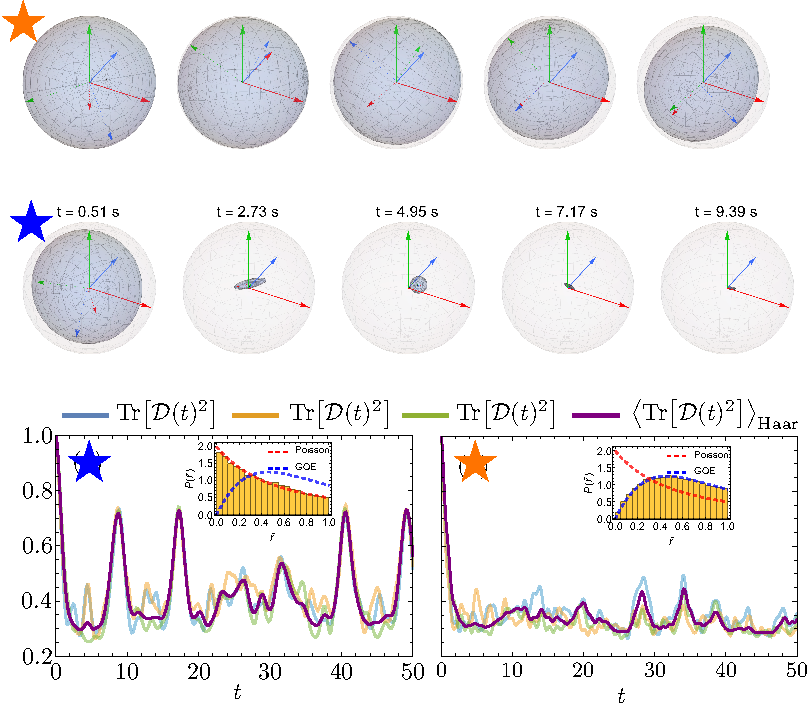
\includegraphics[width=\textwidth]{channel.png}
\end{center}

%\vspace*{-10pt}
%\noindent\textbf{Figure 1.} Energy dissipation: the amplitude damping channel.
%\vspace*{-25pt}
%
%\begin{tikzpicture}[x=1mm,y=1mm,overlay,remember picture]
%\pgftransformshift{\pgfpointanchor{current page}{center}}
%\node[inner sep=0pt] () at (-37, -45) %
%{$\rho \mapsto \mathcal E(\rho)$};
%%
%\node[inner sep=0pt] () at (-37, -85) %
%{$\mcE(\rho) 
%= 
%\Tr_E\qty( e^{-i H t} \rho \otimes \dyad{\psi_E} e^{i H t} )$};
%\end{tikzpicture}
}

\headerbox{Choi-Jamiolkowsky (CJ) matrix $\mathcal D$}
{name=canalesWeyl,
column=0,
below=channels,
span=2}{
%The CJ matrix is a useful representation of a quantum channel $\mathcal E$.
If $\mathcal E$ acts over a $d$-dimensional system, then:
\begin{equation}
\mathcal D
=
\qty( \mathcal E \otimes \one_d )
\qty[ \dyad{\mathrm{Bell}} ].
\end{equation}
Let $\lambda_i$ and $v_i$ be the eigenvalues and eigenvectors reshaped as 
matrices of $\mathcal D$, then:
\begin{equation}
\mathcal E (\rho) 
= 
\sum_i K_i \rho K_i^\dagger,
\quad 
K_i = \sqrt{\lambda_i} v_i
\end{equation}
The purity of $\mathcal D$ has been termed the \textit{unitarity} of 
$\mathcal E$, and $\frac{1}{d^2}
\leq \Tr(\mathcal D^2) = \sum_i \lambda_i^2 \leq 1$.
%\setlist[itemize,1]{left=0pt} 
%\begin{itemize}
%\item  $\mathcal E$ is EB if and only if
%$\big[\mathcal E \otimes \one_B\big](\rho^{AB})$ 
%is separable for any $\rho^{AB}$. \vspace*{-3pt}
%\item $\mathcal E$ is EB if and only if it can be written in \textit{Holevo form}:\vspace*{-3pt}
%\begin{equation}
%\mathcal E(\rho ) = 
%\sum R_k \Tr (F_k \rho ),
%\end{equation}\vspace*{-21pt}
%
%with $R_k$ density matrices and $\{F_k\}$ a POVM.
%\end{itemize}
}

\headerbox{Operational interpretation of $\boldsymbol{\Tr(\mathcal D ^2)}$}
{name= operational-choi,row=0,column=2,span=2}
{\noindent
We show that $\Tr(\mcD^2)$ can be expressed as:
\begin{align}\label{eq:choiPurity:2}
\Tr(\mcD^2) = 
\ev**{
\Tr_S\qty{
U^\dagger 
\Lambda \qty[
U \left( \frac{\one_2}{2} \otimes \dyad{\psi} \right) U^\dagger
]
U
}
}{\psi}.
\end{align}
Thus, it can interpreted as the 
probability of recovering the environment in its initial state after:
\begin{enumerate}
\item evolving forward the joint system, initially in the state 
$\one_S/2 \otimes \dyad{\psi}$, with $U$
\item applying the channel $\Lambda$
\item evolving backward with $U^\dagger$.
\end{enumerate}
}

\headerbox{CJ purity as 
%$\ev{\Tr(\mathcal D ^2)}_{t,\mathrm{Haar}}$
quantum chaos indicator}
{name = chaos-indicator,
column = 2,
below = operational-choi,
span = 2}
{
%\begin{align}\label{eq:haar:avg:choi}
%\underset{\ket{\phi_i} \sim \mu_{\mathrm{Haar}}}
%{\mathbb{E}\qty[\Tr \mcD^2(t)]} 
%= 
%\frac{1}{12^{L-1}} \sum_{\vec{k} \in 
%\{0,1,2,3\}^{L-1}} 3^{\frac{1}{2}\qty(L - 1 - w\qty(\vec{k}))} 
%\Tr \qty[ \Tr_S^2 \qty(U(t) \sigma_{0,\vec{k}}\, U^\dagger(t)) ],
%\end{align}
%\begin{itemize}
%\item $\Tr(\mathcal D ^2)$ depends on $H$, $t$, and 
%$\ket{\psi_E}$, while $\ev{\Tr(\mathcal D ^2)}_{\mathrm{Haar}}$ depends 
%only on $H$ and $t$.
%\end{itemize}
%\vspace*{-5mm}
\begin{center}
\includegraphics[width=\textwidth]{choi_purity.pdf}
\end{center}
\vspace*{-5mm}
%\begin{itemize}
%\item $\ev{\Tr(\mathcal D ^2)}_{t,\mathrm{Haar}}$ is able to resolve the
%integrability-to-chaos transition, when comparing it to the short-range 
%correlations indicator $\ev{\tilde r}$, in a smoother way than previous similar proposed indicator 
%\end{itemize}
\begin{enumerate}
\item[(a)] $H = \sum_{i=1}^L \qty( h_x \sigma_i^x + h_z \sigma_i^z ) 
- J \sum_{i=1}^{L-1} \sigma_i^z \sigma_{i+1}^z$
\item[(b)] $H = \frac{1}{4}\sum_{i=1}^{L-1} \qty[ J_{xy} \qty(\sigma_i^x\sigma_{i+1}^x 
+ \sigma_i^y\sigma_{i+1}^y) + J_z \sigma_i^z\sigma_{i+1}^z ] 
+ \frac{1}{2}\varepsilon \sigma_d^z$
\item[(c)] $H = \frac{1}{4}\sum_{i=1}^{L-1} \qty(\sigma_i^x\sigma_{i+1}^x 
+ \sigma_i^y\sigma_{i+1}^y + \sigma_i^z\sigma_{i+1}^z) 
+ \frac{1}{2}\sum_{i=1}^L h_i \sigma_i^z$
\end{enumerate}
\vspace*{-5mm}
\begin{center}
\includegraphics[width=\textwidth]{r_vs_P_vs_choi-purity.pdf}
\end{center}
}

%\headerbox{Conclusions}
%{name=conclusiones,column=2,below=weylErasing,span=2}{
%\setlist[itemize,1]{left=0pt} 
%\begin{itemize}
%\item We put forward a novel operational interpretation of $\Tr(\mathcal D ^2)$.
%\item $\ev{\Tr(\mathcal D ^2)}_{t,\mathrm{Haar}}$ captures short-range spectral correlations of the total system. What about long-range correlations?
%\end{itemize}
%}

%\headerbox{References}
%{name = referencias,
%column = 2,
%below = chaos-indicator,
%span = 2}{
%%[1] Bengtsson, I., y Zyczkowski, K. (2006). \textit{Geometry of Quantum States: An Introduction to Quantum Entanglement.} Cambridge: Cambridge University Press.
%
%[1] 
%de Leon, J. A., Fonseca, A. Leyvraz, F., Davalos, D., y Pineda, C..
%\textit{Pauli component erasing quantum channels. }
%Phys. Rev. A \textbf{106}, 042604 (2022).
%
%[2] 
%Basile, T., de Leon, J. A., Fonseca, A. Leyvraz, F., y Pineda, C..
%\textit{Weyl channels for multipartite systems}. Phys. Rev. A \textbf{109}, 032607
%(2024).
%}

\end{poster}
\end{document}